\begin{figure}
    \centering
    \begin{subfigure}[b]{0.33\textwidth}
        \centering
        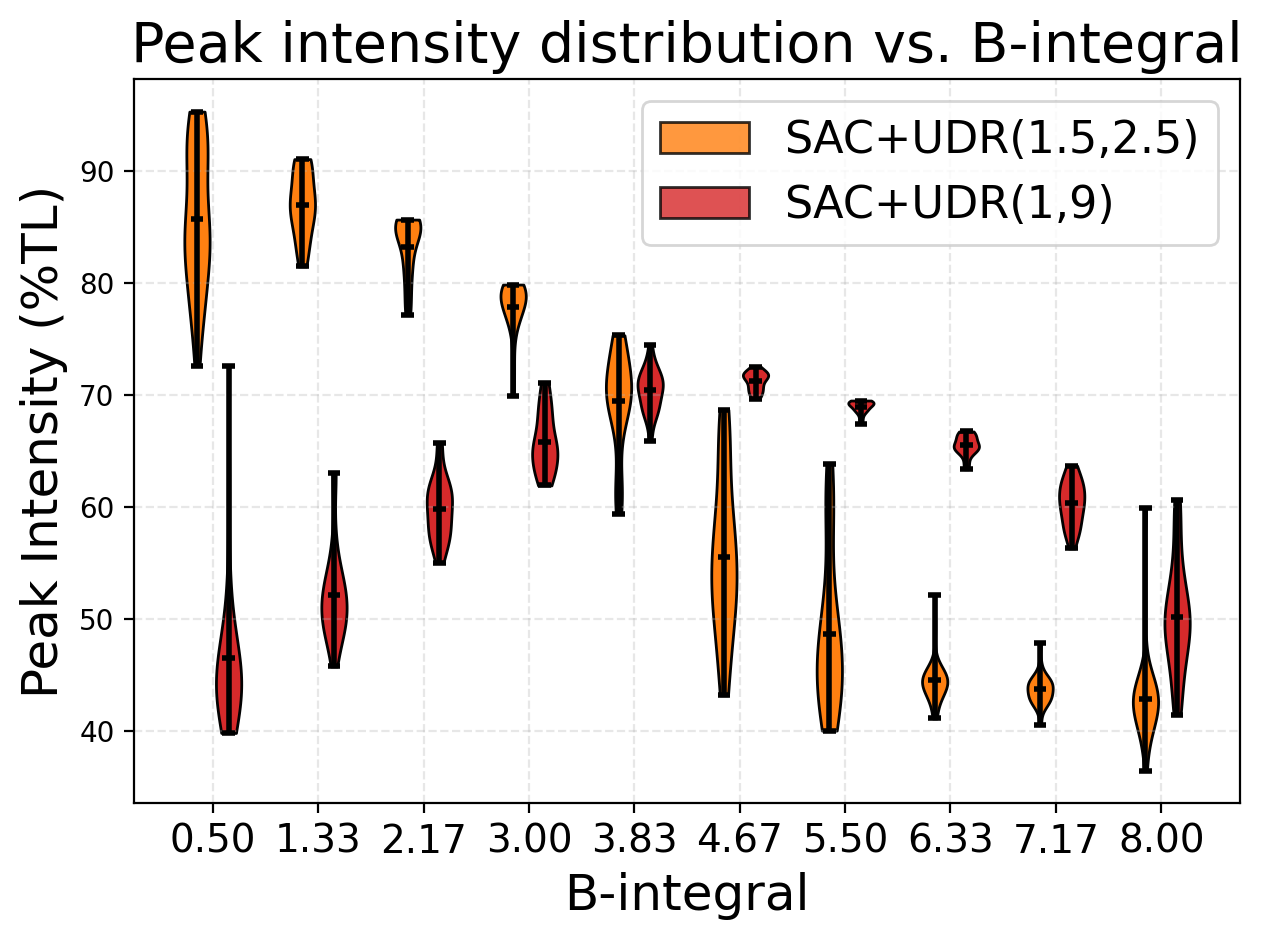
\includegraphics[width=\linewidth]{images/many_udrs_violin.png}
        \caption{\( \mathcal{U}(1.5, 2.5), \ \mathcal{U}(1, 9) \)}
        \label{fig:picking_right_udr_hard}
    \end{subfigure}
    \hfill
    \begin{subfigure}[b]{0.33\textwidth}
        \centering
        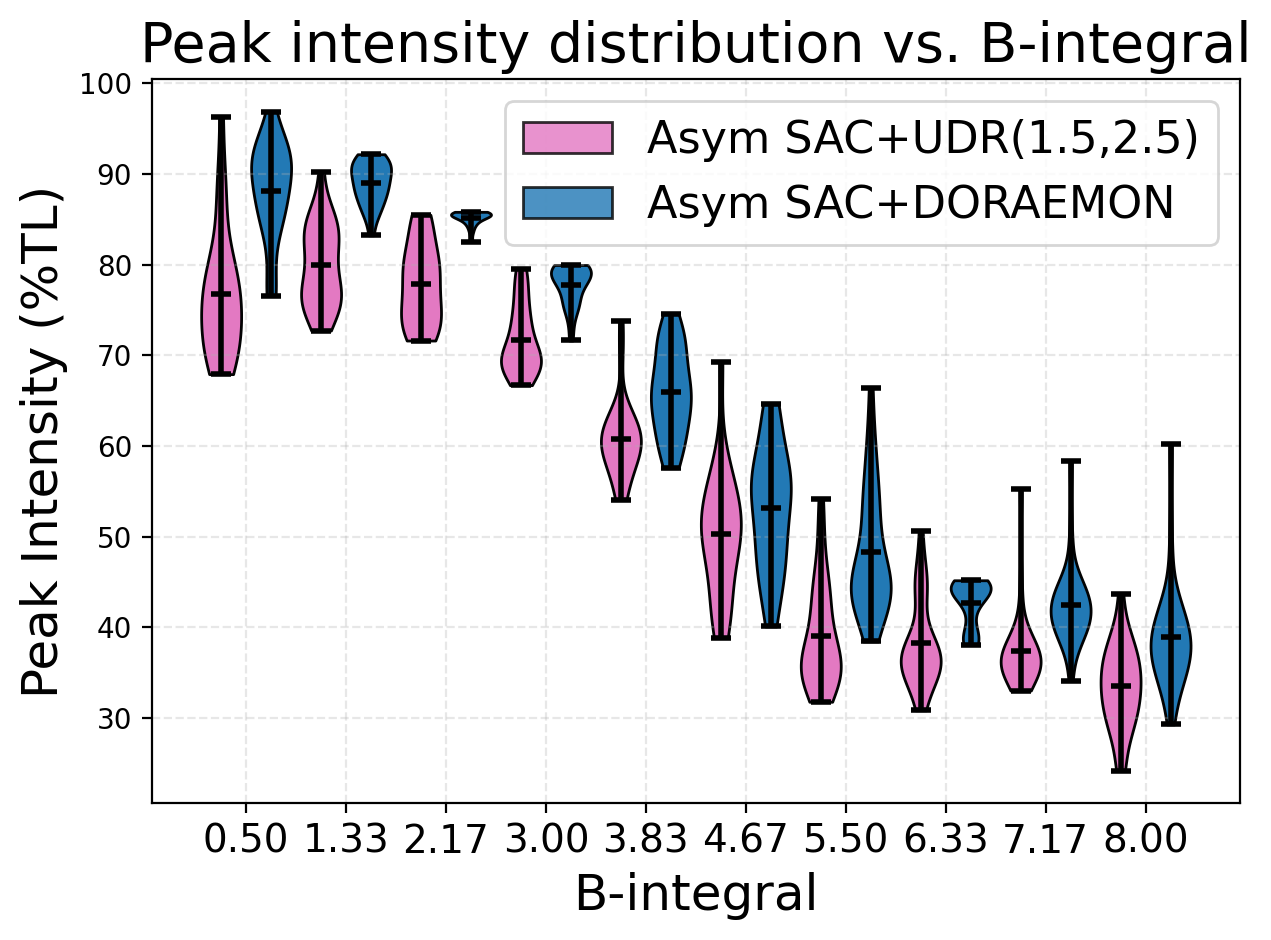
\includegraphics[width=\linewidth]{images/udr_vs_doraemon_violin.png}
        \caption{\( \mathcal{U}(1.5, 2.5) \), DORAEMON} 
        \label{fig:doraemon_outperforms_udr_violin}
    \end{subfigure}
    \hfill
    \begin{subfigure}[b]{0.32\textwidth}
        \centering
        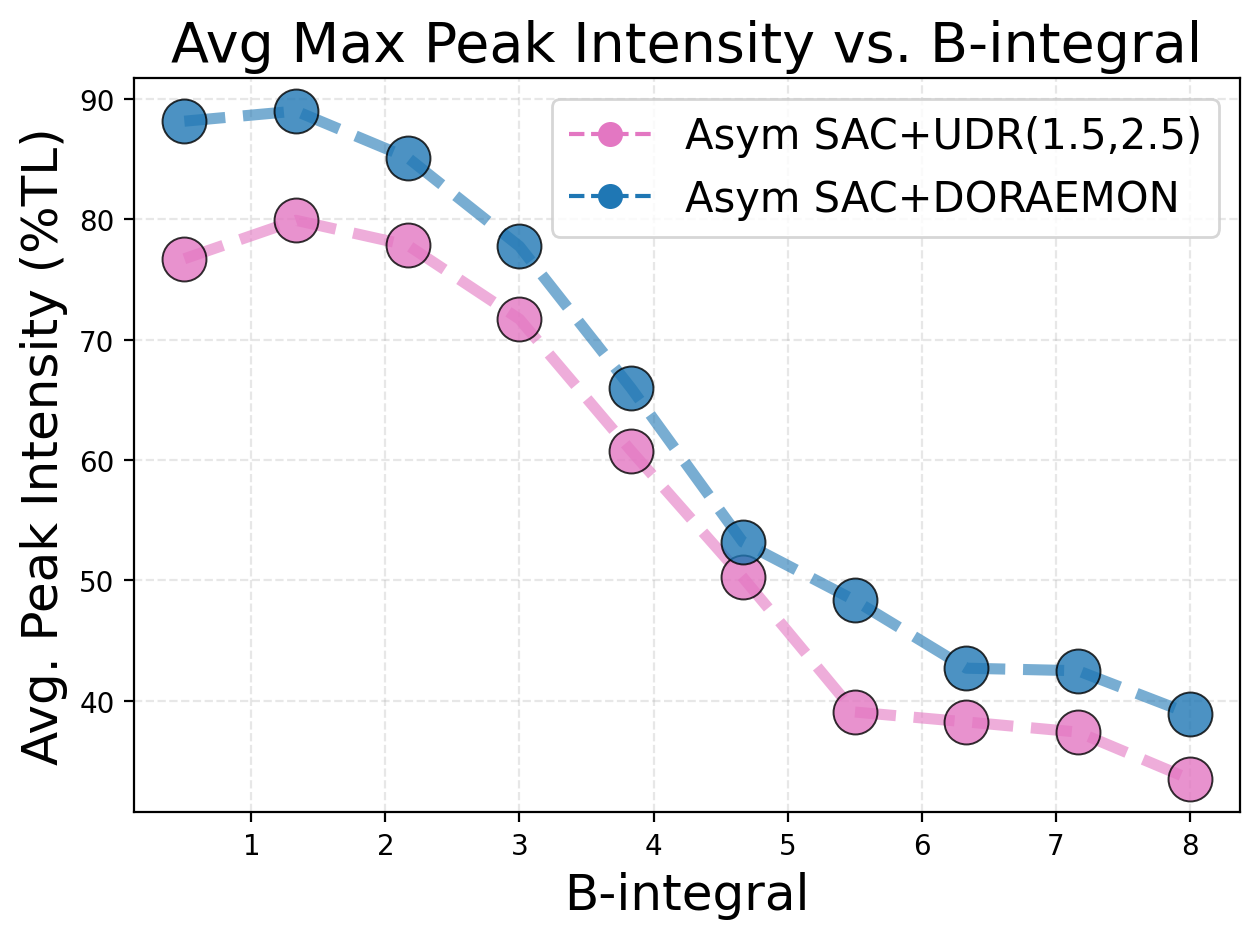
\includegraphics[width=\linewidth]{images/udr_vs_doraemon_average.png}
        \caption{Average \( I^* \) versus \( B \)}
        \label{fig:doraemon_outperforms_udr_scatter}
    \end{subfigure}
    \caption{Distribution (a, b) of and average (c) of \( I^*/I_{TL} \) over 25 test episodes, for policies trained in different setup. Hand-picking the correct distribution for DR is an error prone process (a). Automated approaches like DORAEMON offer a promising alternative adapting the DR distribution using signal from training (b), resulting in an overall better performance over hand-picked distributions across diverse values of \( B \) (c).}
    \label{fig:max_intensity_vs_b_integral}
\end{figure}

\begin{table}
    \centering
    \caption{Success rate over 25 test episodes: proportion of episodes with \( I^* / I_{TL} \geq 70\% \) in multiple experimental conditions}
    \label{tab:succ_rate}
    {%
    \resizebox{0.9\textwidth}{!}{%
    \begin{tabular}{cccccc}
        \textbf{Algorithm} & \textbf{\begin{tabular}[c]{@{}c@{}}Training\\ timesteps\end{tabular}} & \textbf{\begin{tabular}[c]{@{}c@{}}Training\\ Distribution\end{tabular}} & \textbf{\begin{tabular}[c]{@{}c@{}}Success Rate \\ (\(B=0.5\))\end{tabular}} & \textbf{\begin{tabular}[c]{@{}c@{}}Success Rate \\ (\(B=2.17\))\end{tabular}} & \textbf{\begin{tabular}[c]{@{}c@{}}Success Rate \\ (\(B=3.83\))\end{tabular}} \\ \hline
        SAC                & 200k                                                                  & \( \mathcal{U}(1.5, 2.5) \)                                              & 1.00                                                                         & 1.00                                                                          & 0.60                                                                          \\
        \rowcolor[HTML]{EFEFEF} 
        SAC                & 200k                                                                  & \( \mathcal{U}(1, 9) \)                                                  & 0.04                                                                         & 0.00                                                                          & 0.64                                                                          \\
        Asymmetric-SAC     & 200k                                                                  & \( \mathcal{U}(1.5, 2.5) \)                                              & 0.84                                                                         & 1.00                                                                          & 0.08                                                                          \\
        \rowcolor[HTML]{EFEFEF} 
        Asymmetric-SAC     & 200k                                                                  & DORAEMON(1, 3.5)                                                         & 1.00                                                                         & 1.00                                                                          & 0.28                                                                         
    \end{tabular}
    }
    }
\end{table}

We validate our claims on the improved machine-safety of RL over popular baselines such as BO~\citep{shalloo2020automation} by comparing the evolution of the controls applied at test time for both BO and \emph{mini-SAC}. 
As BO cannot be used to process images, we benchmark it against \emph{mini-SAC}, a simplified version of our algorithm that exclusively uses \( \psi \) in the state vector.
We report the comparison between mini-SAC and BO to further show the benefits in terms of machine safety of DRL.
Figure~\ref{fig:bayes_vs_rl} displays the evolution of the controls applied over the first 20 interactions between BO and the RL-based controller. 
Unlike BO's solutions, which are stationary and can only be transferred assuming high-fidelity simulations, RL policies can be transferred across domains.
Notably, this allows us to allocate dangerous erratic exploration to in-simulation training, preventing erratic behavior at test time---similarly to established work in robotics~\citep{kober2013reinforcement}.

\begin{figure}
        \centering
        \begin{minipage}{0.45\textwidth}
            \centering
            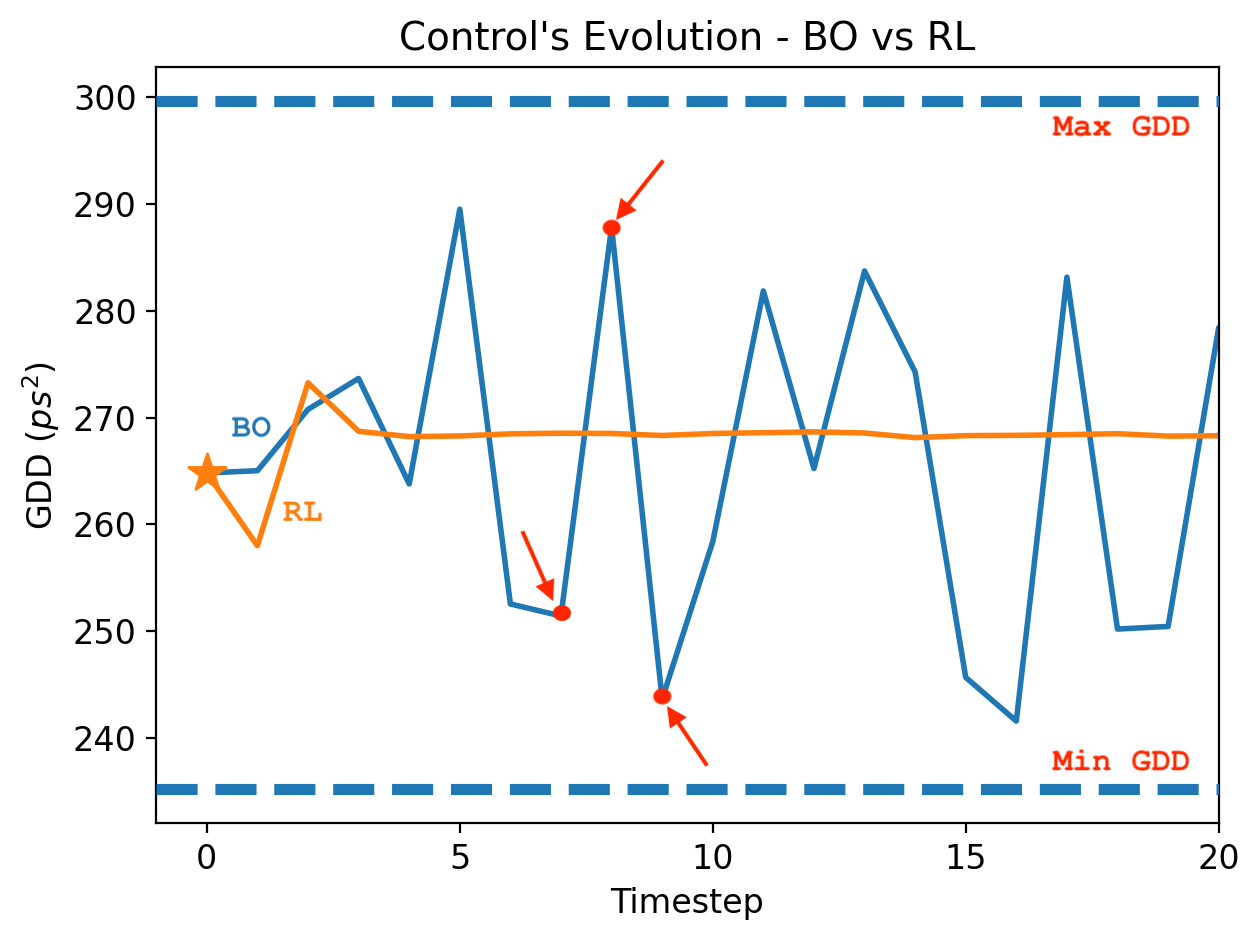
\includegraphics[width=\linewidth]{images/machinesafety.png}
            \caption{Controls applied (BO vs RL). As it samples from an iteratively-refined surrogate model of \(I(\psi)\), BO explores much more erratically than RL.}
            \label{fig:bayes_vs_rl}
        \end{minipage}
        \hfill
        \begin{minipage}{0.45\textwidth}
            \centering
            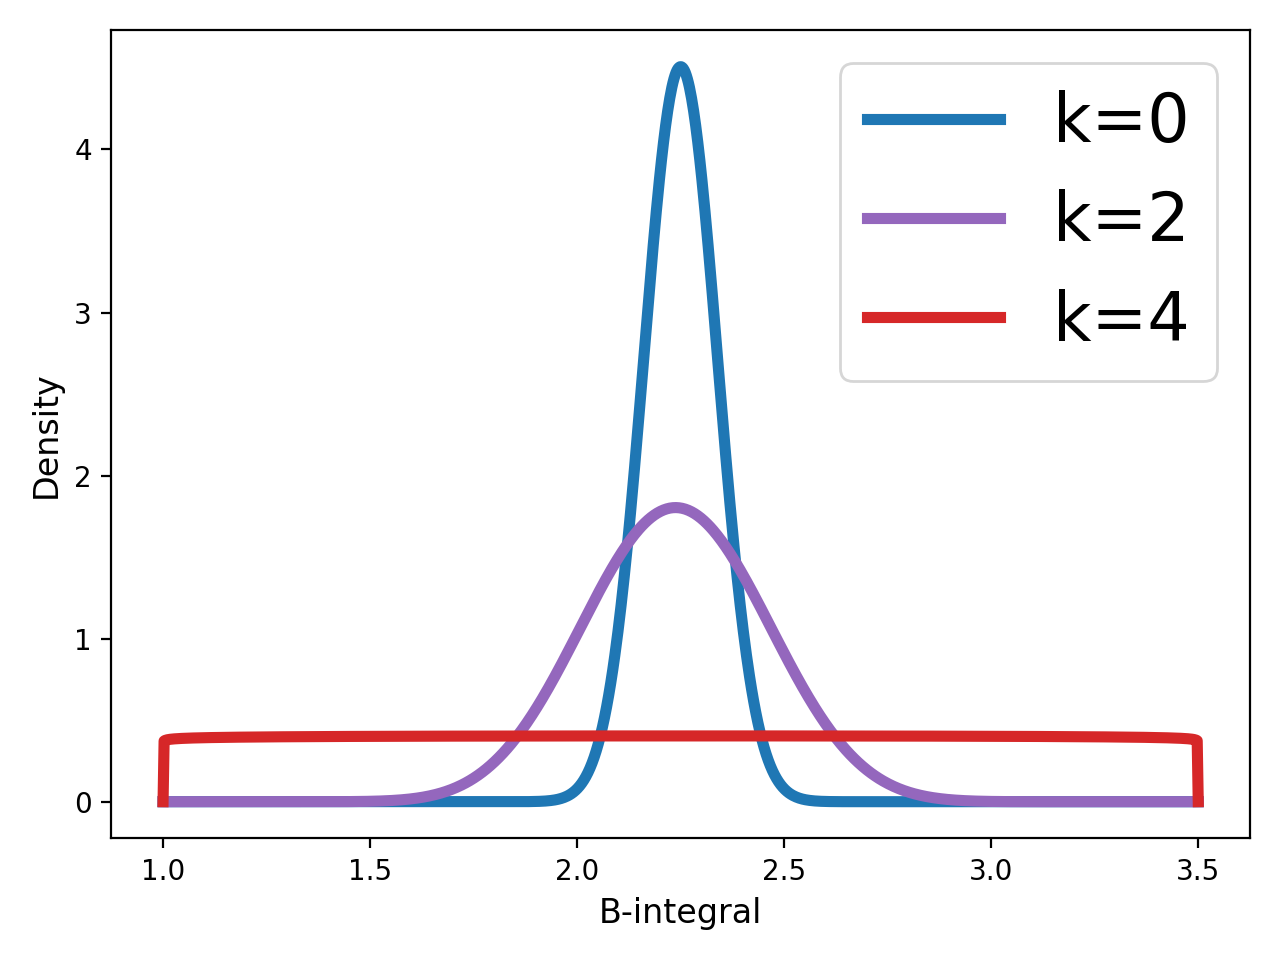
\includegraphics[width=\linewidth]{images/doraemon_distributions_3in1.png}
            \caption{Evolution of the distribution used when training an agent with DORAEMON. Further updates \( k \in [4,20] \) do not impact the evolution of the distribution over \( B \).}
            \label{fig:DORAEMON_distrs_over_training}
        \end{minipage}
        \label{fig:control_and_distribution}
\end{figure}

Since temporal profiles \( \chi(\psi) \) are typically unavailable, we exclusively rely on 64x64 single-channel images as state representations for the agent, as discussed in~\cref{sec:mdp}.
Table~\ref{tab:peak_intensities} shows the average max peak intensity over 25 test episodes, after training SAC for 200k timesteps, while Figure~\ref{fig:frog_opt} shows the FROG traces obtained during a test episode at various timesteps. Crucially, our policy does learn to control \( \psi \) to compress the pulse in time, achieving an average of 85.12\% of TL's peak intensity around \(B_{\text{est}} \), with peaks close to 90\% for oscillations in \( B \) (Table~\ref{tab:max_peak_intensities}). These findings also attest the effectiveness of using single-channel images as affordable proxy input to maximize peak intensity.

\begin{table}
    \centering
    \caption{Average (plus-minus standard deviation) maximal peak intensity over 25 test episodes, for a combination of algorithms, training and testing conditions. We test our algorithms on fixed values of \( B \).
    }
    \label{tab:peak_intensities}
    \resizebox{\textwidth}{!}{%
    \begin{tabular}{cccccc}
        \textbf{Algorithm} & \textbf{\begin{tabular}[c]{@{}c@{}}Training\\ timesteps\end{tabular}} & \textbf{\begin{tabular}[c]{@{}c@{}}Training\\ Distribution\end{tabular}} & \textbf{\begin{tabular}[c]{@{}c@{}}Avg. Max Peak \\ Intensity (\(B=0.5\))\end{tabular}} & \textbf{\begin{tabular}[c]{@{}c@{}}Avg. Max Peak \\ Intensity (\(B=2.17\))\end{tabular}} & \textbf{\begin{tabular}[c]{@{}c@{}}Avg. Max Peak \\ Intensity (\(B=3.83\))\end{tabular}} \\ \hline
        SAC                & 200k                                                                  & \( \mathcal{U}(1.5, 2.5) \)                                              & 85.76 ± 6.19                                                                            & 83.23 ± 2.66                                                                             & 69.49 ± 4.35                                                                             \\
        \rowcolor[HTML]{EFEFEF} 
        SAC                & 200k                                                                  & \( \mathcal{U}(1, 9) \)                                                  & 46.51 ± 6.83                                                                            & 59.87 ± 2.66                                                                             & 70.43 ± 1.87                                                                             \\
        Asymmetric-SAC     & 200k                                                                  & \( \mathcal{U}(1.5, 2.5) \)                                              & 76.73 ± 6.90                                                                            & 77.86 ± 4.38                                                                             & 60.77 ± 4.23                                                                             \\
        \rowcolor[HTML]{EFEFEF} 
        Asymmetric-SAC     & 200k                                                                  & DORAEMON(1, 3.5)                                                         & 88.16 ± 5.22                                                                            & 85.12 ± 0.77                                                                             & 65.98 ± 4.70                                                                            
    \end{tabular}
    }
\end{table}


\begin{figure}
    \centering
    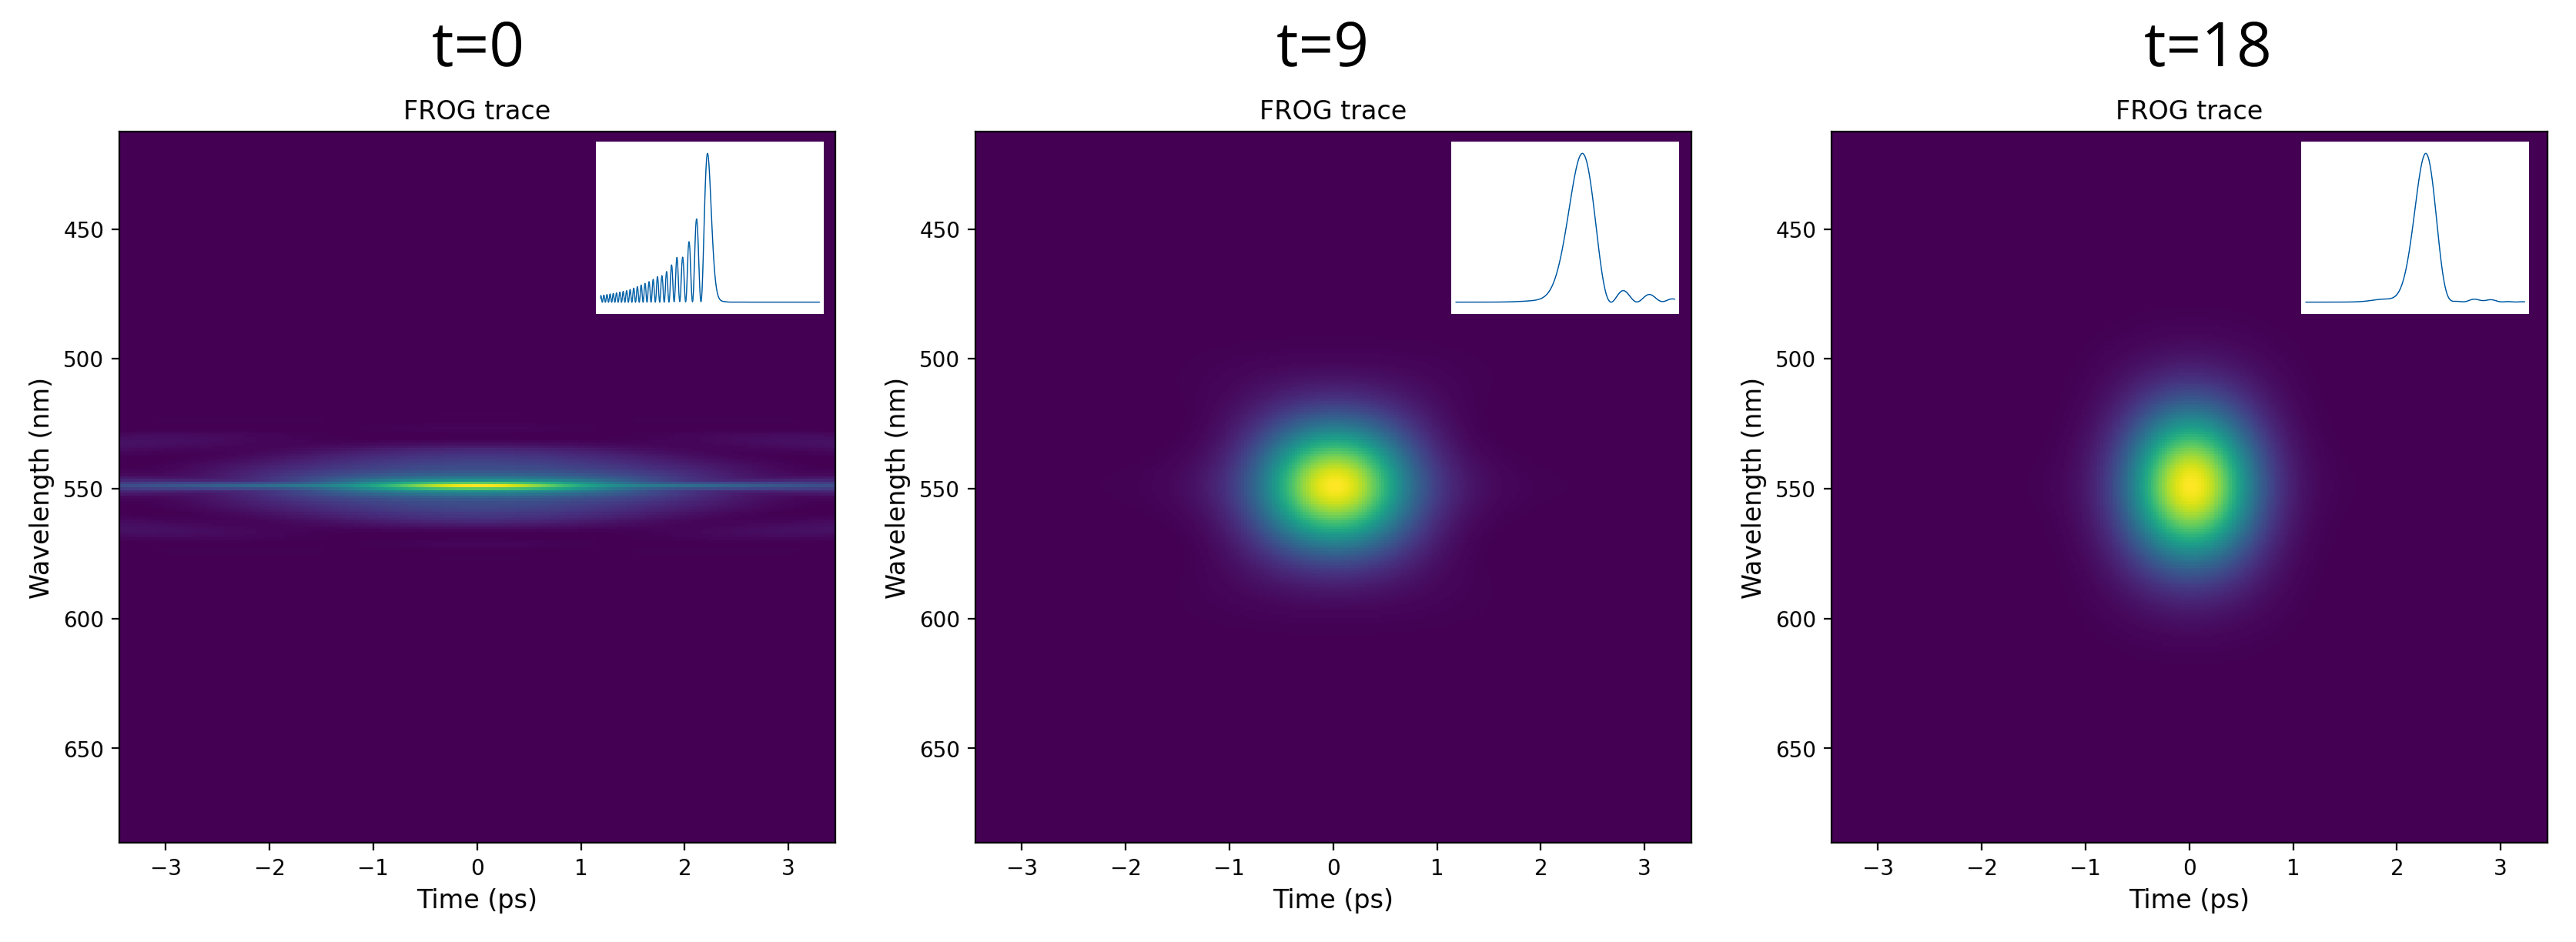
\includegraphics[width=\linewidth]{images/frogopt.png}
    \caption{SAC, learning to shape temporal pulses directly from FROG traces. The temporal profile associated with the FROG trace is superimposed on the top right, and is never made available to the agent. In under 20 interactions, the agent produces near-TL pulses.}
    \label{fig:frog_opt}
\end{figure}
    
    
\begin{figure}
    \centering
    \begin{subfigure}{0.32\textwidth}
        \centering
        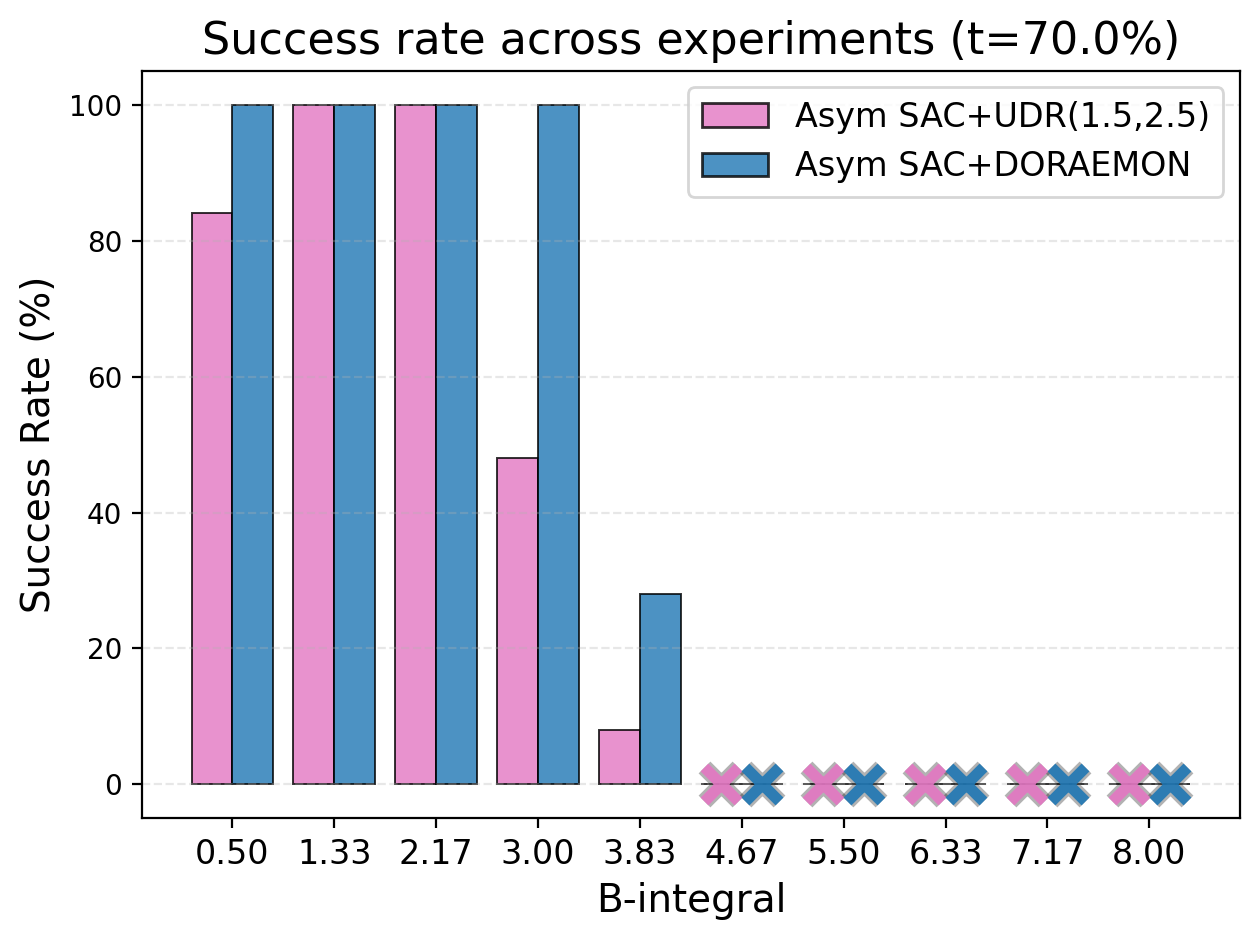
\includegraphics[width=\linewidth]{images/doraemon_vs_udr_succ_rate_70.png}
        \caption{ \( t = 70 \% \) }
        \label{fig:succ_rate_70}
    \end{subfigure}
    \hfill
    \begin{subfigure}{0.32\textwidth}
        \centering
        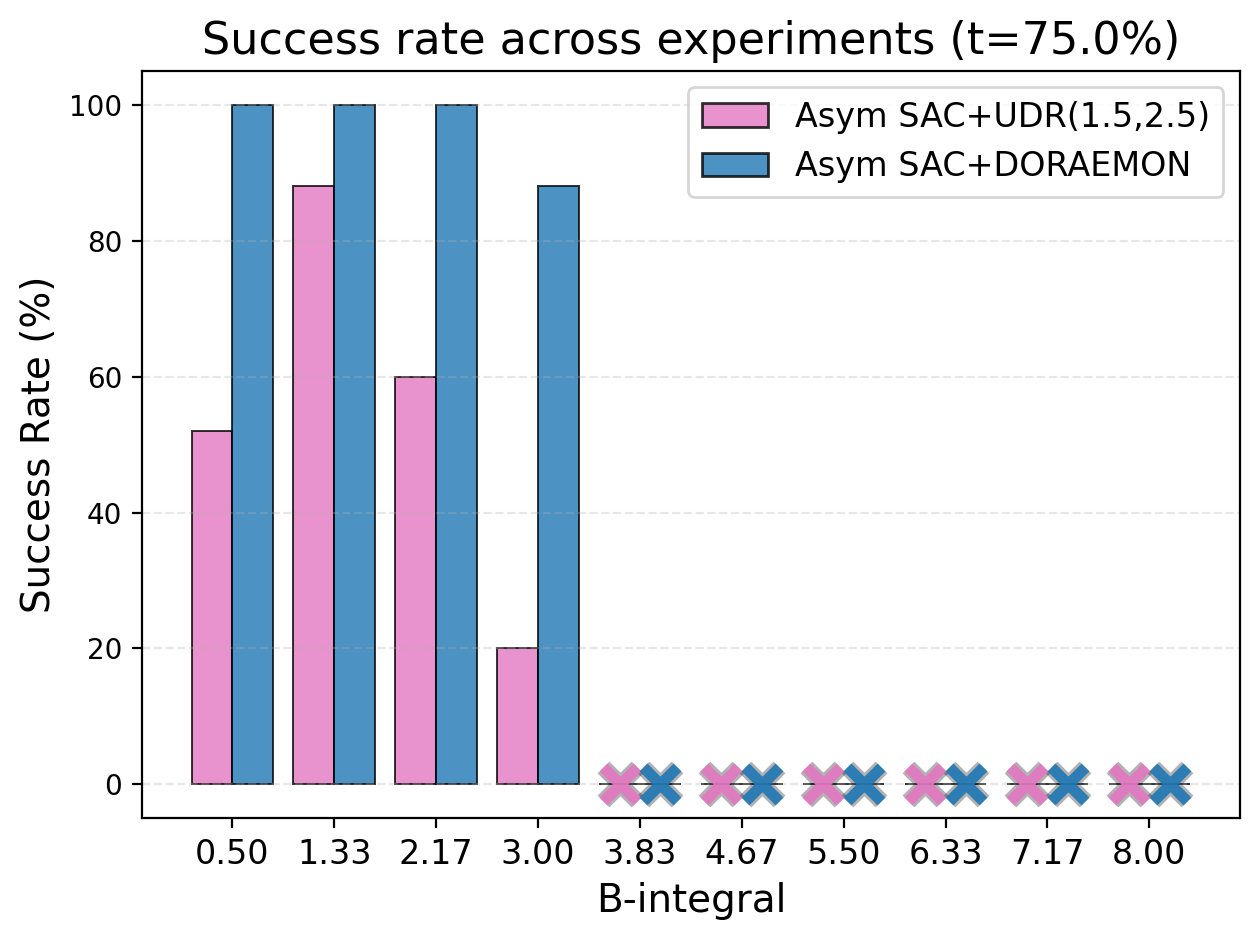
\includegraphics[width=\linewidth]{images/doraemon_vs_udr_succ_rate_75.png}
        \caption{\( t = 75 \% \)} 
        \label{fig:succ_rate_75}
    \end{subfigure}
    \hfill
    \begin{subfigure}{0.32\textwidth}
        \centering
        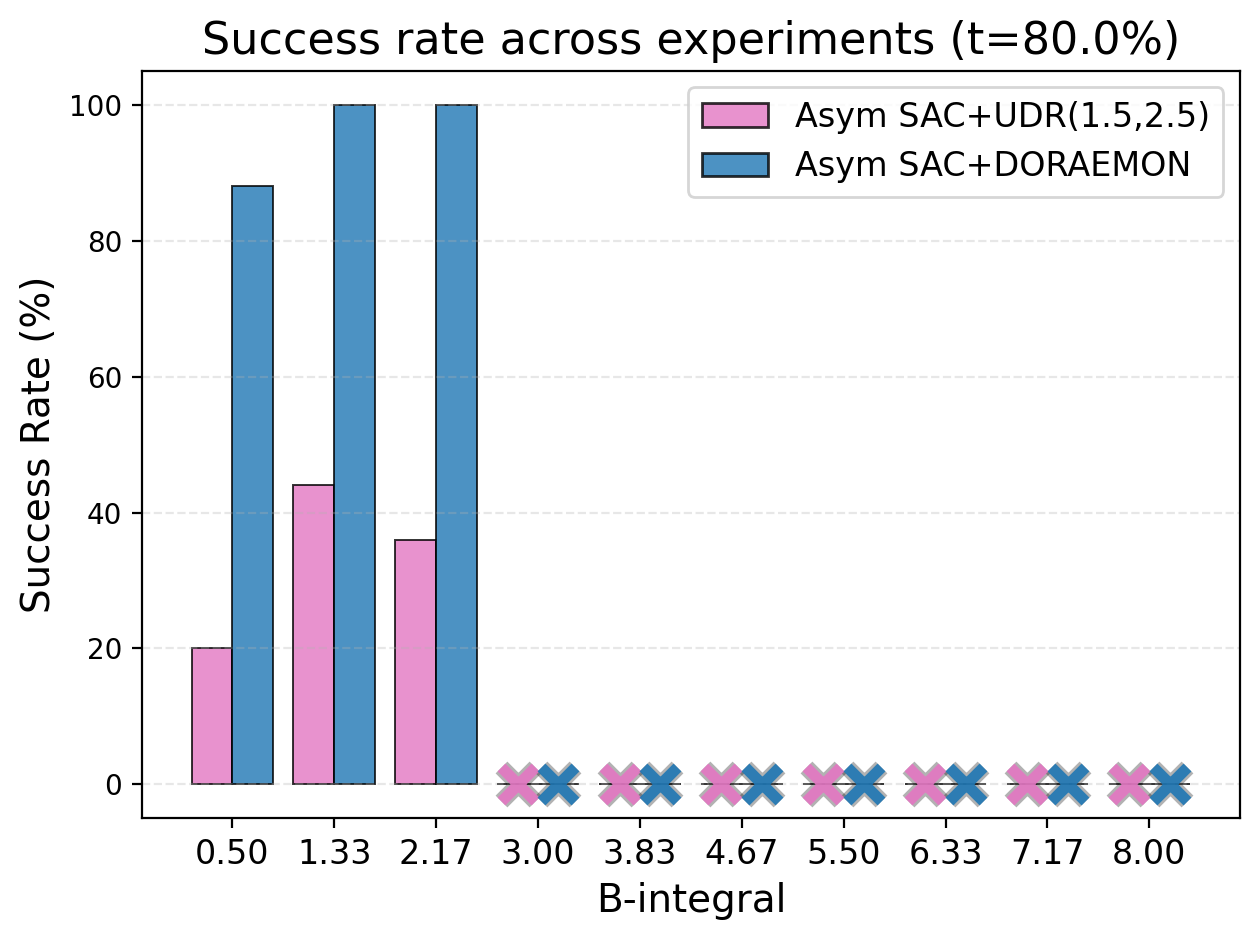
\includegraphics[width=\linewidth]{images/doraemon_vs_udr_succ_rate_80.png}
        \caption{\( t = 80 \% \)}
        \label{fig:succ_rate_80}
    \end{subfigure}
    \caption{Success rates for DORAEMON vs \( \mathcal U(1.5, 2.5) \) across different thresholds. Bars indicates the percentage of the 25 test episodes achieving peak intensities above the specified threshold value. Crosses indicate no test episode achieved \(I^*/I_{TL} \geq t \).}
    \label{fig:succ_rate}
\end{figure}

Later, we benchmark the robustness of our policy to changes in the environment dynamics.
Particularly, we employ DR during training, and use Asymmetric-SAC together with a stack of the last \( n=5 \) states. Using the resulting \emph{history-based} policy holds promise in the context of DR to promote adaptive, meta-learning behavior~\citep{chen2021understanding, tiboni2023domain, akkaya2019solving}.
We evaluate the performance of our method by measuring the average max intensity versus equally-spaced changes in the value of B-integral (Figure~\ref{fig:max_intensity_vs_b_integral}). We then zoom in on the values believed to represent the system's state more realistically, and report in Table~\ref{tab:peak_intensities} the average peak intensity, alongside the standard deviation. Further, we report in Table~\ref{tab:max_peak_intensities} the minimum and maximum peak intensity measured over 25 test episodes.

We observe the performace of policies to significantly vary based on the distribution used while training (Figure~\ref{fig:picking_right_udr_hard}, Figure~\ref{fig:doraemon_outperforms_udr_violin}), motivating the adoption of an automated DR method such as DORAEMON (Figure~\ref{fig:doraemon_outperforms_udr_scatter}).
Table~\ref{tab:peak_intensities} shows the impact of choosing narrower rather than wider bounds for UDR, as we find wider UDR to cause over-regularization, hindering performance.
We compare a naive UDR approach---using realistic bounds suggested by human experts familiar with the system---with DORAEMON, by adapting the training distribution \( \{ \Xi_{k} \}_{k=1}^K\) across \( K=20 \) steps over 200k timesteps. Compared to UDR, DORAEMON displays better test-time performance around our estimate \( B_{\text{est}} = 2 \), and generally provides superior success rate (Table~\ref{tab:succ_rate}).

Figure~\ref{fig:DORAEMON_distrs_over_training} shows the evolution of the distributions generated by DORAEMON \(\{\Beta(a_k, b_k) \}_{k=1}^{K} \) over the course of training. Interestingly, distributions eventually converge to the maximum entropy \( \mathcal U(1, 3.5) \), indicating that sufficient training performance can be maintained even in the extreme case. To investigate the effectiveness of the curriculum for DORAEMON, we then evaluate it against a naive UDR baseline using \( \mathcal U(1.5, 2.5) \)---a range indicated as realistic by domain experts---and observe DORAEMON's superiority in both Figure~\ref{fig:doraemon_outperforms_udr_scatter} and Table~\ref{tab:peak_intensities}.

Lastly, we report the success rates using an indicator function over the peak intensity achieved in a rollout \( I^* \), \(f_t(I^*) = \mathbf{1}_{I^* \geq t} \). We first present success rates for different threshold value \( t \in [70\%, 75\%, 80\%] \) in Figure~\ref{fig:succ_rate} and then for \( t = 70\% \) only in Table~\ref{tab:succ_rate}.
DORAEMON consistently outperforms \( \mathcal{U}(1.5, 2.5) \), underscoring the premise of the method in our context. Further, DORAEMON exhibits stronger performance in settings affected by less evident non-linear effects (\( B \leq 2.5 \)), more often encountered in practice.

\begin{table}
    \centering
    \caption{Min-Max ranges for the maximal peak intensity over 25 test episodes, for a combination of algorithms, training and testing conditions.
    }
    \label{tab:max_peak_intensities}
    \resizebox{\textwidth}{!}{%
    \begin{tabular}{cccccc}
        \textbf{Algorithm} & \textbf{\begin{tabular}[c]{@{}c@{}}Training\\ timesteps\end{tabular}} & \textbf{\begin{tabular}[c]{@{}c@{}}Training\\ Distribution\end{tabular}} & \textbf{\begin{tabular}[c]{@{}c@{}}Min/Max Peak \\ Intensity (\(B=0.5\))\end{tabular}} & \textbf{\begin{tabular}[c]{@{}c@{}}Min/Max Peak \\ Intensity (\(B=2.17\))\end{tabular}} & \textbf{\begin{tabular}[c]{@{}c@{}}Min/Max Peak \\ Intensity (\(B=3.83\))\end{tabular}} \\ \hline
        SAC                & 200k                                                                  & \( \mathcal{U}(1.5, 2.5) \)                                              & 72.63/95.31                                                                            & 77.19/85.67                                                                             & 59.39/75.34                                                                             \\
        \rowcolor[HTML]{EFEFEF} 
        SAC                & 200k                                                                  & \( \mathcal{U}(1, 9) \)                                                  & 39.84/72.60                                                                            & 55.03/65.74                                                                             & 65.90/74.48                                                                             \\
        Asymmetric-SAC     & 200k                                                                  & \( \mathcal{U}(1.5, 2.5) \)                                              & 67.92/96.30                                                                            & 71.62/85.49                                                                             & 54.05/73.75                                                                             \\
        \rowcolor[HTML]{EFEFEF} 
        Asymmetric-SAC     & 200k                                                                  & DORAEMON(1, 3.5)                                                         & 76.57/96.86                                                                            & 82.53/85.81                                                                             & 57.55/74.57                                                                            
    \end{tabular}%
    }
\end{table}